\section{Reshaping two intercepts}\label{sec:reshape}

We now change two intercepts of a simplex while preserving their product.
The support sets need not fill the simplex: the construction applies to any
graded family inside it.  Its algebraic step uses the two branches of a node;
its remaining steps are lattice changes and coordinate compressions.
This follows the planar construction of
\citet[Section~4, Proposition~4.1]{OpenAI2026Higher}, with a formal node
whose branches remain distinct in characteristic two.  The nodal bound,
compressions, and primitive-direction choice also appear in
\citet[Propositions~3.2 and~3.4, Lemma~4.3]{OpenAI2026Surfaces};
we give all the arguments needed here.

\begin{proposition}[Two-intercept reshaping]\label{prop:reshape}
Let $n\ge2$, let $A,B,a_3,\ldots,a_n>0$, and let $(S_N)_{N\ge1}$ be a
graded family of finite subsets of $\Z^n$ satisfying
\[
 S_N\subset N\Delta(A,B,a_3,\ldots,a_n).
\]
Put $H=AB$ and $d=\max\{3/A,2/B\}$.  For every $w>0$ with $dw<1/16$,
there is a graded family $(S'_N)_{N\ge1}$ such that
\[
 S'_N\subset N\Delta(w,H/w,a_3,\ldots,a_n),
 \qquad \#S'_N=\#S_N \quad(N\ge1).
\]
The transformation from $S_N$ to $S'_N$ has backward jet transfer in every
degree.  For $n=2$, the lists $a_3,\ldots,a_n$ are empty.
\end{proposition}

We first prove the nodal bound and then choose the lattice direction that
produces the prescribed intercept $w$.  Throughout this section, $H$ and $d$
have the meanings above, and we put
\begin{equation}\label{eq:reshape-constants}
 W=dH=\max\{2A,3B\},\qquad c=1/d,\qquad
 T=d^2H=\max\{9B/A,4A/B\}\ge6.
\end{equation}
In particular, $cW=H$.

\subsection{The two branches of a node}

For $t>0$, order pairs $(\alpha,\beta)\in\Z_{\ge0}^2$ by the
lexicographic order of $(\alpha+t\beta,\beta)$, as in
Lemma~\ref{lem:exposing-weights}.  We denote the least exponent in this
order by $\nu_t$.

\begin{lemma}[Nodal support bound]\label{lem:nodal-bound}
There are formal coordinates $\xi,\eta$ at the origin of $\A^2_k$ with
\[
 y^2+xy-x^3=\xi\eta
\]
for which the following assertion holds.  Given $t>0$, set
\[
 a=\frac{Wt}{1+t},\qquad b=\frac{W}{1+t},\qquad
 Q=\operatorname{conv}\{(0,0),(a,0),(c,c),(0,b)\}.
\]
If $\kappa\ge0$ and $0\ne f\in k[x,y]$ has all its exponents in
$\kappa\Delta(A,B)$, then its expansion in these coordinates satisfies
$\nu_t(f)\in\kappa Q$.
\end{lemma}

\begin{proof}
Write $g=y^2+xy-x^3$.  The parametrization
\begin{equation}\label{eq:node-parametrization}
 x=v(v+1),\qquad y=v^2(v+1)=vx
\end{equation}
identifies the complement of $x=0$ in $g=0$ with
$\operatorname{Spec}k[v,1/(v(v+1))]$: the inverse is $v=y/x$.
Consequently, a polynomial vanishes under \eqref{eq:node-parametrization}
if and only if it is divisible by $g$.  Indeed, vanishing implies
membership in $(g)$ after inverting $x$, and $g$ is relatively prime to
$x$ in the unique factorization domain $k[x,y]$.

The polynomial $Z^2+Z-x$ has simple roots $0$ and $-1$ modulo $x$.
Hensel lifting gives roots $r_1,r_2\in k[[x]]$ with these respective
constant terms.  Set
\[
 \eta=y-xr_1(x),\qquad \xi=y-xr_2(x).
\]
Their linear terms are $y$ and $y+x$, so they are formal coordinates, and
$\xi\eta=g$.  These assertions also hold in characteristic two: the roots
$0$ and $-1=1$ remain distinct and the linear terms remain independent.
Along \eqref{eq:node-parametrization} near $v=0$, uniqueness of the lifted
root gives $r_1(x(v))=v$, so $\eta=0$ and $\xi$ has order one in $v$.
Near $v=-1$, one similarly has $\xi=0$ and $\eta$ has order one in $v+1$.

Factor $f=g^e f_0$ with $e\ge0$ and $g\nmid f_0$.  Give $x,y$ the
positive weights $1/A,1/B$, and write $\deg_{A,B}$ for the maximum weight
of a polynomial's monomials.  This degree is additive on products,
because their highest weight forms multiply nontrivially.  Moreover,
\[
 \deg_{A,B}(g)=d,
 \qquad \deg_{A,B}(f_0)\le\kappa-ed;
\]
here $1/A+1/B\le\max\{3/A,2/B\}=d$.  Thus $ed\le\kappa$.
The nonzero polynomial
\[
 F_0(v)=f_0\bigl(v(v+1),v^2(v+1)\bigr)
\]
has degree at most $W(\kappa-ed)$, since
\[
 2i+3j\le W(i/A+j/B)
\]
for every monomial $x^iy^j$ of $f_0$.  Its expansions at $v=0$ and
$v=-1$ are both nonzero, since $k[v]$ injects into each completed local
ring.  These expansions are exactly the restrictions of $f_0$ to the
two formal branches described above.

Let $\nu_t(f_0)=(\alpha,\beta)$ and $\mu=\alpha+t\beta$.
Every term of its formal expansion has weight at least $\mu$.
Restricting to $\eta=0$ therefore gives order at least $\mu$ on the branch
at $v=0$; restricting to $\xi=0$ gives order at least $\mu/t$ on the
branch at $v=-1$.  The nonzero polynomial $F_0$ consequently satisfies
\[
 (1+1/t)\mu
 \le \ord_{v=0}(F_0)+\ord_{v=-1}(F_0)
 \le \deg(F_0)\le W(\kappa-ed).
\]
Equivalently, $(\alpha,\beta)\in(\kappa-ed)\Delta(a,b)$.
Because $g=\xi\eta$, multiplicativity of least exponents gives
\[
 \nu_t(f)=(e,e)+\nu_t(f_0)
          =ed(c,c)+\nu_t(f_0)\in\kappa Q.
\]
This also covers $\kappa=0$, when $f$ is constant.
\end{proof}

\subsection{A lattice direction of prescribed height}

Choose $t>T$.  With $a,b$ as in Lemma~\ref{lem:nodal-bound}, one has
\[
 a+b=W,\qquad
 \frac ca+\frac cb=\frac{(1+t)^2}{Tt}>1.
\]
Thus $Q$ is a quadrilateral with the vertices in the order displayed in
that lemma, and its area is $c(a+b)/2=H/2$.  The shear
$(\alpha,\beta)\mapsto(\alpha-\beta,\beta)$ sends its vertices to
\[
 (0,0),\quad(a,0),\quad(0,c),\quad(-b,b).
\]
Its vertical slice at horizontal coordinate $q$ has length
\begin{equation}\label{eq:first-slice-length}
 \begin{cases}
 c(1+q/b),&-b\le q\le0,\\
 c(1-q/a),&0\le q\le a.
 \end{cases}
\end{equation}
Compression in the second coordinate therefore places the support in the
triangle
\begin{equation}\label{eq:reshape-triangle}
 P=\operatorname{conv}\{(-b,0),(a,0),(0,c)\}.
\end{equation}
Its area is again $H/2$; see Figure~\ref{fig:reshape-polygons}.

\begin{figure}[tbp]
\centering
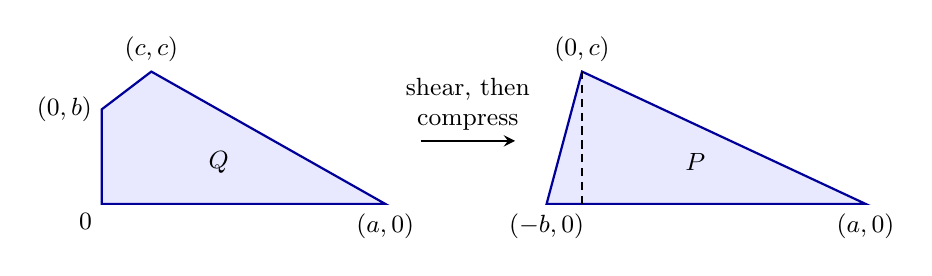
\begin{tikzpicture}[font=\small,>=stealth]
 \begin{scope}[xscale=.9,yscale=2.4]
  \filldraw[fill=blue!9,draw=blue!60!black,thick]
   (0,0)--(4,0)--(.7,.7)--(0,.5)--cycle;
  \node[below left] at (0,0) {$0$};
  \node[below] at (4,0) {$(a,0)$};
  \node[above] at (.7,.7) {$(c,c)$};
  \node[left] at (0,.5) {$(0,b)$};
  \node at (1.65,.22) {$Q$};
 \end{scope}
 \draw[->,thick] (4.05,.8)--(5.25,.8)
  node[midway,above,align=center] {shear, then\\compress};
 \begin{scope}[shift={(6.1,0)},xscale=.9,yscale=2.4]
  \filldraw[fill=blue!9,draw=blue!60!black,thick]
   (-.5,0)--(4,0)--(0,.7)--cycle;
  \draw[densely dashed] (0,0)--(0,.7);
  \node[below] at (-.5,0) {$(-b,0)$};
  \node[below] at (4,0) {$(a,0)$};
  \node[above] at (0,.7) {$(0,c)$};
  \node at (1.6,.22) {$P$};
 \end{scope}
\end{tikzpicture}
\caption{The nodal bound $Q$ becomes the triangle $P$ after a shear and
vertical compression.  Each vertical slice of the sheared bounding polygon
is replaced by an interval of the same length starting at zero;
Formula~\eqref{eq:first-slice-length}
gives the resulting boundary.  Both polygons have area $H/2$.  The drawing
is schematic; the displayed vertex coordinates are exact.}
\label{fig:reshape-polygons}
\end{figure}

The next lemma chooses both $t$ and a primitive lattice direction.  We
seek unimodular coordinates in which $P$ has vertical extent $H/w$;
its area $H/2$ will then force its largest horizontal slice to have
length $w$.

\begin{lemma}[Prescribed primitive height]\label{lem:primitive-height}
If $w>0$ and $dw<1/16$, there exist $t>T$ and a primitive vector
$u=(i,j)\in\Z^2$ such that the three vertex heights
$z\mapsto\det(u,z)$ of the triangle $P$ in
\eqref{eq:reshape-triangle} are distinct and their range has length $H/w$.
\end{lemma}

\begin{proof}
Put $R=H/w$ and $a_0=WT/(1+T)$.  As $t$ ranges over $(T,\infty)$,
the value $a=Wt/(1+t)$ ranges over $(a_0,W)$.
For $u=(i,j)$, the heights of $(-b,0),(a,0),(0,c)$ are $jb,-ja,i/d$.
We seek $j>0$ and $i$ such that
\[
 ja+i/d=R,\qquad i/d>jb.
\]
The first equality turns the second inequality into $R-jW>0$.
Thus we first choose $jW\le R/2$, and then use the freedom in $a$ to
obtain the equality with $i$ coprime to $j$.

Take $j$ to be the largest power of two at most
\[
 \frac{R}{2W}=\frac{1}{2dw}.
\]
Then $j>1/(4dw)>4$.  The open interval
\[
 \bigl(d(R-jW),\ d(R-ja_0)\bigr)
\]
has length
\[
 dj(W-a_0)=\frac{jT}{1+T}>2,
\]
so it contains an odd integer $i$.  Since $j$ is a power of two, $(i,j)$
is primitive.  There is a unique $t>T$ such that
\[
 a=\frac{R-i/d}{j}\in(a_0,W).
\]
The resulting heights satisfy
\[
 -ja<jb<i/d,\qquad
 i/d-jb=R-jW\ge R/2>0,\qquad i/d+ja=R.
\]
This gives the required height range and distinctness.
\end{proof}

\subsection{Completion of the transformation}

\begin{proof}[Proof of Proposition~\ref{prop:reshape}]
Fix $t$ and $u$ from Lemma~\ref{lem:primitive-height}; these choices will
be used in every degree.  Keep coordinates $3,\ldots,n$ unchanged.
For each degree $N$ and each label
$\gamma=(\gamma_3,\ldots,\gamma_n)$ occurring in $S_N$, put
\[
 \kappa=N-\sum_{h=3}^n\frac{\gamma_h}{a_h}\ge0.
\]
The pair exponents with this label lie in $\kappa\Delta(A,B)$.
Take their polynomial span in $k[x,y]$ and replace it by its least
exponents in the coordinates $\xi,\eta$ and order $\nu_t$.
Lemma~\ref{lem:least-terms} preserves cardinality and gradedness: the row
spaces multiply into the row with degree and label added, and the same
coordinates and order are used throughout.  For fixed $N$, choose a basis
with distinct least exponents in each row and apply
Lemma~\ref{lem:exposing-weights} to the finite union of these bases.
Its common weight vector allows Lemma~\ref{lem:formal-transfer} to apply
to all labels at once, giving backward jet transfer.  The old points can
be chosen in the dense open torus of $\A^2\times\T^{n-2}$.

Lemma~\ref{lem:nodal-bound} places the new pair exponents in $\kappa Q$.
Apply the shear above and compress in the second coordinate.
Lemmas~\ref{lem:unimodular} and~\ref{lem:compression}, together with
\eqref{eq:first-slice-length}, give the bound $\kappa P$.
It remains to turn this triangle into $\Delta(w,H/w)$.

Complete the primitive vector $u$ to an integral basis $(u,v)$ with
$\det(u,v)=1$, and use the coordinates in that basis.  This is a
unimodular change, and its second coordinate is precisely
$z\mapsto\det(u,z)$.  Write $q_0<q_1<q_2$ for the three vertex heights of
the transformed triangle.  Its horizontal slice length is linear from
zero at $q_0$ to a maximum at $q_1$, and linear back to zero at $q_2$.
The maximum is $w$, since area is preserved and
\[
 \frac H2=\frac12(q_2-q_0)\,\bigl(\text{maximum slice length}\bigr),
 \qquad q_2-q_0=R=H/w.
\]
Compressing in the first coordinate therefore gives the bound
\[
 \operatorname{conv}\{(0,q_0),(w,q_1),(0,q_2)\}.
\]
Its vertical slice at first coordinate $h\in[0,w]$ has length
$R(1-h/w)$.  Compression in the second coordinate gives
$\Delta(w,R)$, as illustrated in Figure~\ref{fig:final-compression}.  These slice statements commute with multiplication by
$\kappa$, so the resulting pair bound is $\kappa\Delta(w,R)$ for every
label.  If $\kappa=0$, its only possible pair exponent is $(0,0)$, which
remains unchanged at every step.

Restoring the labels gives
$S'_N\subset N\Delta(w,R,a_3,\ldots,a_n)$.  Every step preserves
cardinality and gradedness and has backward jet transfer, so their
composition has all the asserted properties.
\end{proof}


\begin{figure}[tbp]
\centering
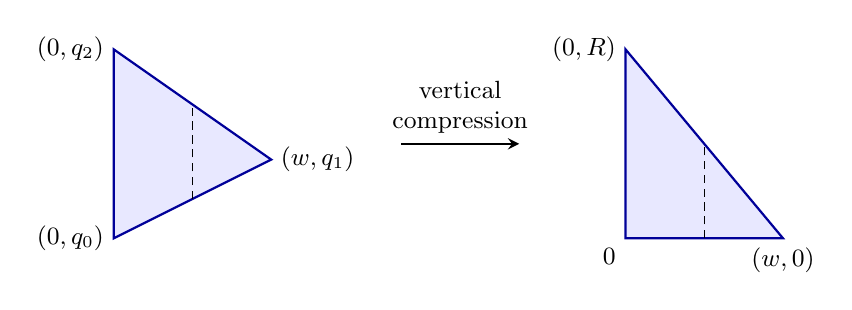
\begin{tikzpicture}[font=\small,>=stealth]
 \begin{scope}
  \filldraw[fill=blue!9,draw=blue!60!black,thick]
   (0,-.6)--(2,.4)--(0,1.8)--cycle;
  \draw[densely dashed] (1,-.1)--(1,1.1);
  \node[left] at (0,-.6) {$(0,q_0)$};
  \node[left] at (0,1.8) {$(0,q_2)$};
  \node[right] at (2,.4) {$(w,q_1)$};
 \end{scope}
 \draw[->,thick] (3.65,.6)--(5.15,.6)
  node[midway,above,align=center] {vertical\\compression};
 \begin{scope}[shift={(6.5,-.6)}]
  \filldraw[fill=blue!9,draw=blue!60!black,thick]
   (0,0)--(2,0)--(0,2.4)--cycle;
  \draw[densely dashed] (1,0)--(1,1.2);
  \node[below left] at (0,0) {$0$};
  \node[below] at (2,0) {$(w,0)$};
  \node[left] at (0,2.4) {$(0,R)$};
 \end{scope}
\end{tikzpicture}
\caption{After the lattice change and horizontal compression, a final
vertical compression produces the target triangle.  At first coordinate
$h$, both vertical slices have length $R(1-h/w)$, where
$R=q_2-q_0=H/w$.  Dashed segments mark corresponding slices.}
\label{fig:final-compression}
\end{figure}
